\documentclass[10pt,a4paper]{jsarticle}
\usepackage{listings}
\usepackage{fancyhdr}
\usepackage{lastpage}
\usepackage[dvipdfmx]{graphicx}

\lhead{プログラミング実習IIレポート(第4回)}
\rhead{学籍番号:201811433 氏名:西田 直人}
\cfoot{\thepage/\pageref{LastPage}}

\pagestyle{fancy}

\title{プログラミングII実習レポート課題第4回}
\author{西田直人}

\begin{document}
%\markright{プログラミング実習1Aレポート(第1回) 学籍番号:201811433 氏名:西田直人}
%\maketitle
\begin{center}
{\LARGE プログラミング実習IIレポート課題第4回} \\
\large
西田直人 \\ 2018年12月14日
\end{center}
\normalsize
\section{課題4-1}
\noindent a.

\subsection{source}
\lstinputlisting[basicstyle=\ttfamily\footnotesize,frame=single]{a4-1a.c}

\subsection{result}

\begin{lstlisting}[basicstyle=\ttfamily\footnotesize,frame=single]
  s1811433@7C202-P048:~/prog2/04/04kadai$ cc -o a4-1a a4-1a.c
  s1811433@7C202-P048:~/prog2/04/04kadai$ ./a4-1a
  0: isalpha, 1: isdigit, 2: islower, 3: isupper ? 0
  char = a
  'a' is an alphabet
  s1811433@7C202-P048:~/prog2/04/04kadai$ ./a4-1a
  0: isalpha, 1: isdigit, 2: islower, 3: isupper ? 1
  char = 3
  '3' is a digit
  s1811433@7C202-P048:~/prog2/04/04kadai$ ./a4-1a
  0: isalpha, 1: isdigit, 2: islower, 3: isupper ? 2
  char = a
  'a' is lowercase
  s1811433@7C202-P048:~/prog2/04/04kadai$ ./a4-1a
  0: isalpha, 1: isdigit, 2: islower, 3: isupper ? 3
  char = A
  'A' is uppercase
  s1811433@7C202-P048:~/prog2/04/04kadai$ ./a4-1a
  0: isalpha, 1: isdigit, 2: islower, 3: isupper ? 0
  char = A
  'A' is an alphabet
  s1811433@7C202-P048:~/prog2/04/04kadai$ ./a4-1a
  0: isalpha, 1: isdigit, 2: islower, 3: isupper ? 0
  char = 1
  '1' is NOT an alphabet
  s1811433@7C202-P048:~/prog2/04/04kadai$ ./a4-1a
  0: isalpha, 1: isdigit, 2: islower, 3: isupper ? 1
  char = A
  'A' is NOT a digit
  s1811433@7C202-P048:~/prog2/04/04kadai$ ./a4-1a
  0: isalpha, 1: isdigit, 2: islower, 3: isupper ? 1
  char = a
  'a' is NOT a digit
  s1811433@7C202-P048:~/prog2/04/04kadai$ ./a4-1a
  0: isalpha, 1: isdigit, 2: islower, 3: isupper ? 2
  char = A
  'A' is NOT lowercase
  s1811433@7C202-P048:~/prog2/04/04kadai$ ./a4-1a
  0: isalpha, 1: isdigit, 2: islower, 3: isupper ? 2
  char = 1
  '1' is NOT lowercase
  s1811433@7C202-P048:~/prog2/04/04kadai$ ./a4-1a
  0: isalpha, 1: isdigit, 2: islower, 3: isupper ? 3
  char = A
  'A' is uppercase
  s1811433@7C202-P048:~/prog2/04/04kadai$ ./a4-1a
  0: isalpha, 1: isdigit, 2: islower, 3: isupper ? 3
  char = a
  'a' is NOT uppercase
  s1811433@7C202-P048:~/prog2/04/04kadai$ ./a4-1a
  0: isalpha, 1: isdigit, 2: islower, 3: isupper ? 3
  char = 1
  '1' is NOT uppercase
  s1811433@7C202-P048:~/prog2/04/04kadai$ 
\end{lstlisting}

\b.

\subsection{source}
\lstinputlisting[basicstyle=\ttfamily\footnotesize,frame=single]{check_char.c}

\subsection{result}

\begin{lstlisting}[basicstyle=\ttfamily\footnotesize,frame=single]
  s1811433@7C202-P048:~/prog2/04/04kadai$ cc -o check_char check_char.c
  s1811433@7C202-P048:~/prog2/04/04kadai$ ./check_char
  Usage: ./check_char -adlu char
  s1811433@7C202-P048:~/prog2/04/04kadai$ ./check_char -a 0
  '0' is NOT an alphabet
  s1811433@7C202-P048:~/prog2/04/04kadai$ ./check_char -a a
  'a' is an alphabet
  s1811433@7C202-P048:~/prog2/04/04kadai$ ./check_char -a A
  'A' is an alphabet
  s1811433@7C202-P048:~/prog2/04/04kadai$ ./check_char -d 1
  '1' is a digit
  s1811433@7C202-P048:~/prog2/04/04kadai$ ./check_char -d A
  'A' is NOT a digit
  s1811433@7C202-P048:~/prog2/04/04kadai$ ./check_char -d a
  'a' is NOT a digit
  s1811433@7C202-P048:~/prog2/04/04kadai$ ./check_char -l a
  'a' is lowercase
  s1811433@7C202-P048:~/prog2/04/04kadai$ ./check_char -l 1
  '1' is NOT lowercase
  s1811433@7C202-P048:~/prog2/04/04kadai$ ./check_char -l A
  'A' is NOT lowercase
  s1811433@7C202-P048:~/prog2/04/04kadai$ ./check_char -u a
  'a' is NOT uppercase
  s1811433@7C202-P048:~/prog2/04/04kadai$ ./check_char -u A
  'A' is uppercase
  s1811433@7C202-P048:~/prog2/04/04kadai$ ./check_char -u 1
  '1' is NOT uppercase
  s1811433@7C202-P048:~/prog2/04/04kadai$ ./check_char -e 3
  Error: unknown option: -e.
  Usage: ./check_char -adlu char
  s1811433@7C202-P048:~/prog2/04/04kadai$
  
\end{lstlisting}


\section{課題4-2}
\noindent a.
\subsection{source}
\lstinputlisting[basicstyle=\ttfamily\footnotesize,frame=single]{a4-2.c}


\subsection{result}
\begin{lstlisting}[basicstyle=\ttfamily\footnotesize,frame=single]
  s1811433@7C202-P048:~/prog2/04/04kadai$ cc -o a4-2 a4-2.c -lm
  s1811433@7C202-P048:~/prog2/04/04kadai$ ./a4-2
  0: sin, 1: cos, 2: tan ? 0
  theta = 3.14159265358979
  sin(theta) = 0.000000
  s1811433@7C202-P048:~/prog2/04/04kadai$ ./a4-2
  0: sin, 1: cos, 2: tan ? 1
  theta = 1.0471955
  cos(theta) = 0.500002
  s1811433@7C202-P048:~/prog2/04/04kadai$ ./a4-2
  0: sin, 1: cos, 2: tan ? 1
  theta = 1.04719755
  cos(theta) = 0.500000
  s1811433@7C202-P048:~/prog2/04/04kadai$ ./a4-2
  0: sin, 1: cos, 2: tan ? 2
  theta = 0.78539816
  tan(theta) = 1.000000
  s1811433@7C202-P048:~/prog2/04/04kadai$ ./a4-2
  0: sin, 1: cos, 2: tan ? 0
  theta = 0
  sin(theta) = 0.000000
  s1811433@7C202-P048:~/prog2/04/04kadai$ ./a4-2
  0: sin, 1: cos, 2: tan ? 0
  theta = 1
  sin(theta) = 0.841471
  s1811433@7C202-P048:~/prog2/04/04kadai$ ./a4-2
  0: sin, 1: cos, 2: tan ? 1
  theta = 0
  cos(theta) = 1.000000
  s1811433@7C202-P048:~/prog2/04/04kadai$ ./a4-2
  0: sin, 1: cos, 2: tan ? 2
  theta = 1
  tan(theta) = 1.557408
  s1811433@7C202-P048:~/prog2/04/04kadai$
  
\end{lstlisting}

b.
\subsection{source}
\lstinputlisting[basicstyle=\ttfamily\footnotesize,frame=single]{trigonometric_arg.c}


\subsection{result}
\begin{lstlisting}[basicstyle=\ttfamily\footnotesize,frame=single]
  s1811433@7C202-P048:~/prog2/04/04kadai$ cc -o trigonometric_arg trigonometric_arg.c -lm
  s1811433@7C202-P048:~/prog2/04/04kadai$ ./trigonometric_arg -a 3
  Error: unknown or invalid option.
  Usage: ./trigonometric_arg -sct double [-rd]
  -s: sin
  -c: cos
  -t: tan
  -r: radian (default)
  -d: degree
  s1811433@7C202-P048:~/prog2/04/04kadai$ ./trigonometric_arg -s 30 -d
  sin(30.000000) = 0.500000
  s1811433@7C202-P048:~/prog2/04/04kadai$ ./trigonometric_arg -r -c 0.78539816325
  cos(0.785398) = 0.707107
  s1811433@7C202-P048:~/prog2/04/04kadai$ ./trigonometric_arg -c 0.78539816325
  cos(0.785398) = 0.707107
  s1811433@7C202-P048:~/prog2/04/04kadai$ ./trigonometric_arg -t 45 -d
  tan(45.000000) = 1.000000
  s1811433@7C202-P048:~/prog2/04/04kadai$ ./trigonometric_arg -s 90
  sin(90.000000) = 0.893997
  s1811433@7C202-P048:~/prog2/04/04kadai$ ./trigonometric_arg -s 90 -d
  sin(90.000000) = 1.000000
  s1811433@7C202-P048:~/prog2/04/04kadai$
  
\end{lstlisting}


\section{課題4-3}
\subsection{source}
\lstinputlisting[basicstyle=\ttfamily\footnotesize,frame=single]{filter_array.c}

\subsection{result}

\begin{lstlisting}[basicstyle=\ttfamily\footnotesize,frame=single]
  s1811433@7C202-P048:~/prog2/04/04kadai$ cc -o filter_array filter_array.c -lm
  s1811433@7C202-P048:~/prog2/04/04kadai$ ./filter_array 10
  input (10 integers):
  747,986,169,441,426,941,73,377,802,265

  square numbers (2 integers):
  169,441

  prime numbers (2 integers):
  941,73

  power of two (0 integers):
  s1811433@7C202-P048:~/prog2/04/04kadai$ ./filter_array 30
  input (30 integers):
  747,986,169,441,426,941,73,377,802,265,
  859,925,394,740,603,842,265,976,202,896,
  516,143,439,259,274,648,886,938,469,799

  square numbers (2 integers):
  169,441

  prime numbers (4 integers):
  941,73,859,439

  power of two (0 integers):
  s1811433@7C202-P048:~/prog2/04/04kadai$ ./filter_array 300
  input (300 integers):
  747,986,169,441,426,941,73,377,802,265,
  859,925,394,740,603,842,265,976,202,896,
  516,143,439,259,274,648,886,938,469,799,
  455,215,137,975,7,562,916,79,291,69,
  695,149,993,88,889,948,282,153,923,483,
  400,790,625,838,49,898,837,286,187,305,
  436,642,872,572,968,878,134,883,309,424,
  951,3,924,296,91,812,243,372,316,517,
  854,67,307,478,905,707,727,741,992,914,
  398,427,907,269,999,874,146,484,757,806,
  907,59,809,830,354,899,994,948,622,661,
  817,475,728,123,304,984,181,382,724,172,
  295,473,950,553,741,948,427,239,431,535,
  44,689,945,852,871,299,102,216,246,723,
  228,414,549,955,536,204,290,716,586,14,
  239,232,838,189,785,579,488,563,169,271,
  449,212,311,393,416,533,691,869,748,289,
  944,328,702,844,634,590,48,924,657,985,
  289,248,216,126,436,352,704,275,914,872,
  545,714,436,208,107,851,740,149,71,840,
  789,14,167,843,858,800,432,257,723,440,
  241,11,687,456,137,474,160,192,101,425,
  64,645,139,851,852,245,53,944,745,123,
  783,534,489,949,376,346,748,159,602,823,
  950,842,833,989,649,321,462,808,513,562,
  233,928,559,371,778,762,967,830,705,711,
  304,839,596,792,787,323,489,887,481,90,
  709,783,283,893,771,932,214,584,91,78,
  498,675,5,408,45,134,169,363,315,226,
  426,618,64,21,762,203,344,250,441,176

  square numbers (13 integers):
  169,441,400,625,49,484,169,289,289,64,
  169,64,441

  prime numbers (49 integers):
  941,73,859,439,137,7,79,149,883,3,
  67,307,727,907,269,757,907,59,809,661,
  181,239,431,239,563,271,449,311,691,107,
  149,71,167,257,241,11,137,101,139,53,
  823,233,967,839,787,887,709,283,5

  power of two (2 integers):
  64,64
  s1811433@7C202-P048:~/prog2/04/04kadai$ ./filter_array 810
  input (810 integers):
  747,986,169,441,426,941,73,377,802,265,
  859,925,394,740,603,842,265,976,202,896,
  516,143,439,259,274,648,886,938,469,799,
  455,215,137,975,7,562,916,79,291,69,
  695,149,993,88,889,948,282,153,923,483,
  400,790,625,838,49,898,837,286,187,305,
  436,642,872,572,968,878,134,883,309,424,
  951,3,924,296,91,812,243,372,316,517,
  854,67,307,478,905,707,727,741,992,914,
  398,427,907,269,999,874,146,484,757,806,
  907,59,809,830,354,899,994,948,622,661,
  817,475,728,123,304,984,181,382,724,172,
  295,473,950,553,741,948,427,239,431,535,
  44,689,945,852,871,299,102,216,246,723,
  228,414,549,955,536,204,290,716,586,14,
  239,232,838,189,785,579,488,563,169,271,
  449,212,311,393,416,533,691,869,748,289,
  944,328,702,844,634,590,48,924,657,985,
  289,248,216,126,436,352,704,275,914,872,
  545,714,436,208,107,851,740,149,71,840,
  789,14,167,843,858,800,432,257,723,440,
  241,11,687,456,137,474,160,192,101,425,
  64,645,139,851,852,245,53,944,745,123,
  783,534,489,949,376,346,748,159,602,823,
  950,842,833,989,649,321,462,808,513,562,
  233,928,559,371,778,762,967,830,705,711,
  304,839,596,792,787,323,489,887,481,90,
  709,783,283,893,771,932,214,584,91,78,
  498,675,5,408,45,134,169,363,315,226,
  426,618,64,21,762,203,344,250,441,176,
  692,501,958,974,393,80,257,958,664,700,
  35,513,374,391,920,771,876,440,133,190,
  665,558,160,81,931,921,635,626,522,75,
  153,213,575,463,539,319,542,795,277,557,
  846,663,69,220,406,988,990,281,780,122,
  823,444,32,334,876,314,254,510,939,127,
  936,91,340,510,905,230,829,447,24,457,
  355,222,119,424,441,876,763,430,509,542,
  903,331,338,286,664,213,599,269,75,889,
  395,10,332,86,872,236,315,700,682,691,
  156,37,912,626,812,704,502,574,485,362,
  468,387,692,805,673,707,369,623,975,795,
  512,721,157,195,159,28,430,825,79,464,
  515,586,852,778,563,663,833,416,588,317,
  777,407,704,468,563,728,174,284,702,500,
  78,565,573,586,759,731,613,189,555,43,
  652,422,628,855,551,191,869,384,606,456,
  700,383,215,755,202,777,482,728,60,536,
  227,490,100,799,75,859,529,40,47,436,
  82,50,857,62,904,759,604,772,142,561,
  579,194,943,793,948,497,922,782,224,981,
  317,802,822,416,601,897,626,481,288,24,
  268,369,73,476,782,328,235,385,451,728,
  946,382,921,240,174,221,88,447,354,311,
  780,670,465,601,437,65,497,415,897,784,
  438,517,505,511,992,286,190,578,23,641,
  306,968,22,578,559,547,150,647,994,503,
  309,773,172,773,373,961,189,222,375,438,
  357,812,954,213,674,297,851,864,875,873,
  856,532,192,877,109,102,775,611,748,120,
  113,409,892,637,181,617,597,370,190,323,
  807,898,486,112,111,512,408,313,375,282,
  537,582,813,728,810,274,181,584,884,281,
  704,996,689,947,984,869,915,580,590,104,
  254,396,354,740,507,816,251,267,128,977,
  548,664,910,713,743,719,338,275,302,573,
  555,5,920,243,304,904,112,218,483,53,
  674,89,449,27,180,307,842,782,573,321,
  758,473,336,667,185,78,737,874,352,38,
  446,259,395,365,501,698,268,964,267,103,
  17,940,191,817,318,722,475,511,503,48,
  183,612,872,518,630,408,947,366,281,299,
  403,726,557,149,442,409,198,710,373,465,
  164,389,756,706,557,426,427,31,288,929,
  430,471,540,301,988,521,708,935,886,988,
  585,640,65,493,141,859,901,338,568,273,
  154,83,13,262,788,921,687,566,952,974,
  494,381,796,385,682,784,257,741,718,142,
  81,302,133,497,794,273,355,46,611,274,
  671,116,356,35,377,495,956,415,60,907,
  741,905,639,536,641,320,319,897,413,388

  square numbers (21 integers):
  169,441,400,625,49,484,169,289,289,64,
  169,64,441,81,441,100,529,784,961,784,
  81

  prime numbers (131 integers):
  941,73,859,439,137,7,79,149,883,3,
  67,307,727,907,269,757,907,59,809,661,
  181,239,431,239,563,271,449,311,691,107,
  149,71,167,257,241,11,137,101,139,53,
  823,233,967,839,787,887,709,283,5,257,
  463,277,557,281,823,127,829,457,509,331,
  599,269,691,37,673,157,79,563,317,563,
  613,43,191,383,227,859,47,857,317,601,
  73,311,601,23,641,547,647,503,773,773,
  373,877,109,113,409,181,617,313,181,281,
  947,251,977,743,719,5,53,89,449,307,
  103,17,191,503,947,281,557,149,409,373,
  389,557,31,929,521,859,83,13,257,907,
  641

  power of two (6 integers):
  64,64,32,512,512,128
  s1811433@7C202-P048:~/prog2/04/04kadai$
  
\end{lstlisting}

\subsection{課題4-4}

\subsubsection{source}
\lstinputlisting[basicstyle=\ttfamily\footnotesize,frame=single]{filter_array.c\
a4-4(Submission).c}

\subsubsection{result}
\noindent BEFORE\\
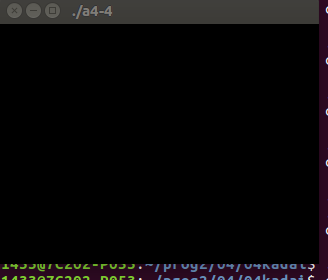
\includegraphics[width=5cm]{before.png}

\noindent AFTER CLICKING BY A MOUSE\\
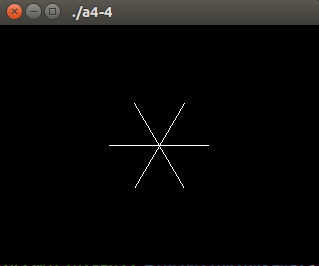
\includegraphics[width=5cm]{mouse.png}


\noindent AFTER ENTERING A KEY\\
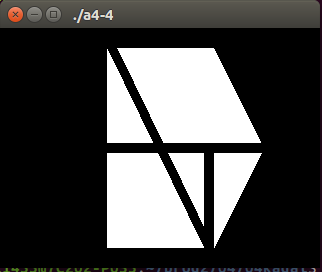
\includegraphics[width=5cm]{key.png}

\end{document}
